\documentclass[letterpaper,10pt]{article}
\usepackage[utf8]{inputenc}
\usepackage{graphicx}
\graphicspath{{./static/images/}}

%opening
\title{Control Methodologies for the Mars Rover Lab}
\author{Martin Jay McKee}
\date{}

\begin{document}

\maketitle

\begin{abstract}
  The goal of this project is to provide a new control system for the version 2 Mars Robotics Laboratory (MRL) rovers.  The first section of this document introduces the current control system for the MRL rovers.  The second section outlines control issues that the author has noticed as being particularly frustrating to users of the MRL.  The third section outlines some potential interfaces which could be used as a replacement to the current design.  Additionally, advantages and disadvantages are introduced.  The final section describes potential additions to the MRL systems which would improve the safety or functionality of the system above and beyond simple changes to the control methodology.
\end{abstract}

\section{Lego Mindstorms Software}
  The current control system is an unmodified installation of the Lego Mindstorms software within which a simple program with a run block and motor block are linked.  The rover is then controlled by adjusting three parameters: steering, power and rotations.  The steering and power values range from -100 to 100 while the rotations parameters can, for all intents and purposes, be anything\footnote{It is, actually, at least $-1^{37}$ to $1^{38}$}.  If either power or rotations (but not both) are negative, the rover will go backward and otherwise the rover moves forward.  Steering works by changing the rotations of the left- and right-hand motors relative to the commanded rotations.  Power is somewhere between controlling motor speed and torque.  It is not clear what it does, in general.  However, when the wheels are spinning in soft ground, decreasing the power reduces the slippage.
  
\section{Typical Control Issues}
  There are a number of issues that users generally have with the current control system.  They are outlined here in related sections.
  
  \subsection{Software Issues}
    \subsubsection{Hanging}
      There are times where the software locks-up, typically when a command is being downloaded to the rover.  When this happens users generally ask for help and are delayed until an MRL volunteer is able to assist them.  In some cases, users will leave if they are delayed too long.
      
    \subsubsection{(Mental) Sandbox too Big}
      Because the Mindstorms software is a general-purpose programming environment, it is possible for users to modify the program\dots{}adding to it or breaking it up.  Both possibilities are typically detrimental to the enjoyment of the general public.  This stems from the fact that such changes are generally unintended and they make the rovers appear to ``break''.  If nothing else, it causes users to become frustrated .  It also wastes volunteers' time because the are often required to ``fix'' the system.
      
    \subsubsection{Lack of Limits}
      The fact that there are essentially no limits of the commands makes it very likely for users to enter commands that get the rovers in trouble.  On the one hand, they can drive the rover much further than intended and get them stuck.  On the other, it is not atypical for users to enter a rediculous number of rotations -- say 1,000,000 -- which cuases the rover to become unresponsive for a long period.  Either users ask for assistance or they leave due to the rovers ``not working''.
      
    \subsection{Lack or Responsiveness}
      The Lego Mindstorms software can feel unresponsive in a number of ways.  If the rover is unable to complete a command, it will continue trying until it reaches the goal.  While it displays a pushable ``stop'' button.  It is very small and is not noticed by users.  In this case, the rover will also flash the activity LED (unless the user has changed the programming so that the activity LED functions in a different manner).  
  
  \subsection{Control Corner Cases}
    \subsubsection{Direction Control}
      If either the power or rotations are negative then the rover will go in reverse.  If they are both negative (or both positive) the rover will go forward.  This actually makes sense if these values are, somehow, multiplicitive.  It doesn't seem to be intuitive to most users however.  It is pretty simple to keep users from tripping over this by simply not telling them that rotations can be negative, however, that is hardly a good solution overall.
      
    \subsubsection{Power Selection and Command End}
      It is very easy to lock up the current rovers with a command input.  By commanding the rover to move at all and setting the power to zero.  This, again, makes perfect sense.  If the rover is told to turn the wheels one revolution but to not use any power doing it, the paradox is apparent.  Users of all ages, however, are caught out by this quirk.  Moreover, it is surprisingly difficult to explain the problem to many people.
      
  \subsection{Physical Issues}
    \subsubsection{Where's the front?}
      Users are so used to seeing standard children's tricycles and adult tricycle motorcycles that they will actually argue with volunteers that the single freewheel ``is'' the front of the rover and that it doesn't go forward like it should.  Telling them that the two large wheels are the front is typically sufficient for adults but may not be for children.  By simply representing the shape of the rover on the interface and drawing an arrow representing the commanded motion, this problem may be reduced regardless of the shape of the new rover.
      
    \subsubsection{Motor Power}
      Ideally the rovers need to be a bit more powerful.  When the Lego rovers have fresh batteries and motors, they work very well.  As the systems age, however, the begin to be stopped by even very small bumps on the ground.  When the rovers begin to get stuck on every little thing, users become -- understandably -- annoyed and will sometimes leave as a result of it.  Even if speeds are internally limited, the version 2 rovers should have higher power capabilities to allow for power loss with age and wear.
      
\section{Interface Ideas}
  Before we look at the interface ideas, there are a couple of very important things to remember.  First, the colors used in these sketches are for ease of viewing, not because they are a good color scheme for a final system.  A more subtle and unified color scheme is going to be important.  It will be especially important to limit contrast except where necessary to make certain indications most visible.  For the time being, however, using these high-contrast diagrams makes sense.  Secondly, these drawings are deliberately quick and dirty.  Rather than spend a lot of time trying to work out the most beautiful solution, these drawings simply get a quick sketch of the idea on paper.  A much more polished design is going to be necessary.
  
  Another thing to keep in mind is that it is going to be important to have these interfaces adapt to the display device if possible.  By changing the iPads from landscape to portrait the controls will, ideally, change configuration in such a way that they are most visible and understandable.  Very likely, this adaptation is going to have to be, at least in part, manual.
  
  \subsection{Seperated Power, Steering and Distance Controls}
    This is just the same as the Mindstorms control system that is in use now.  However, it would allow us to add limits and remove corner cases.  There are two primary advantages to this interface design.  First, it is very simple to implement.  Standard HTML form components would be enough to get a working version of this running.  As a result, it should be quick to run on the client side and use minimal resources on both the server and client.  The second advantage of this interface design is that -- being the closest to the current interface -- it would require the smallest adjustment for the educational classes with more advanced students.
  
    The basic interface might look something like the following:
    
    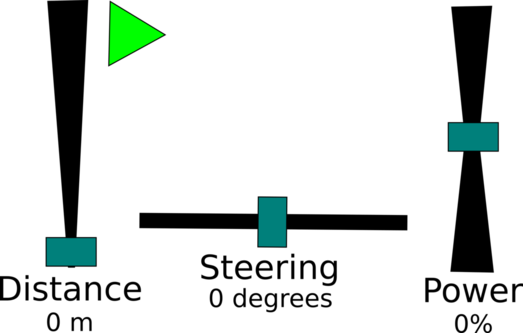
\includegraphics[width=8cm]{seperated_neutral}

    On the far left is a slider that sets the distance to be traveled in the next command -- up to some standard limit.  One primary advantage of this design is that it reduces the possibility of commanding too long of travel.  Bottom center is a steering control which has maximum limits of plus or minus 360 degrees (one full rotation).  If the distance is set to zero, then the rover will still pivot in place.  At the far right, there is a power control.  The power control does two things: it sets the speed at which the rover will move and it sets the direction.  Motor torque should be autonomously controlled to minimize wheel slippage.  Because the power control does double duty, it may prove to be difficult to use and it might be beneficial to seperate the power and direction functionality.  Then again, that would lead to four controls that need to be taught to users at the beginning.  Also visible in this image are the green ``drive'' button and an open area that will typically house an arrow that describes the motion to be completed.  Once pressed, the green button is replaced with a red ``stop'' button as long as the rover is moving.  Also, the arrow is progressively filled to show the progress of the movement.  
    
    Let's examine a command using this interface:
    
    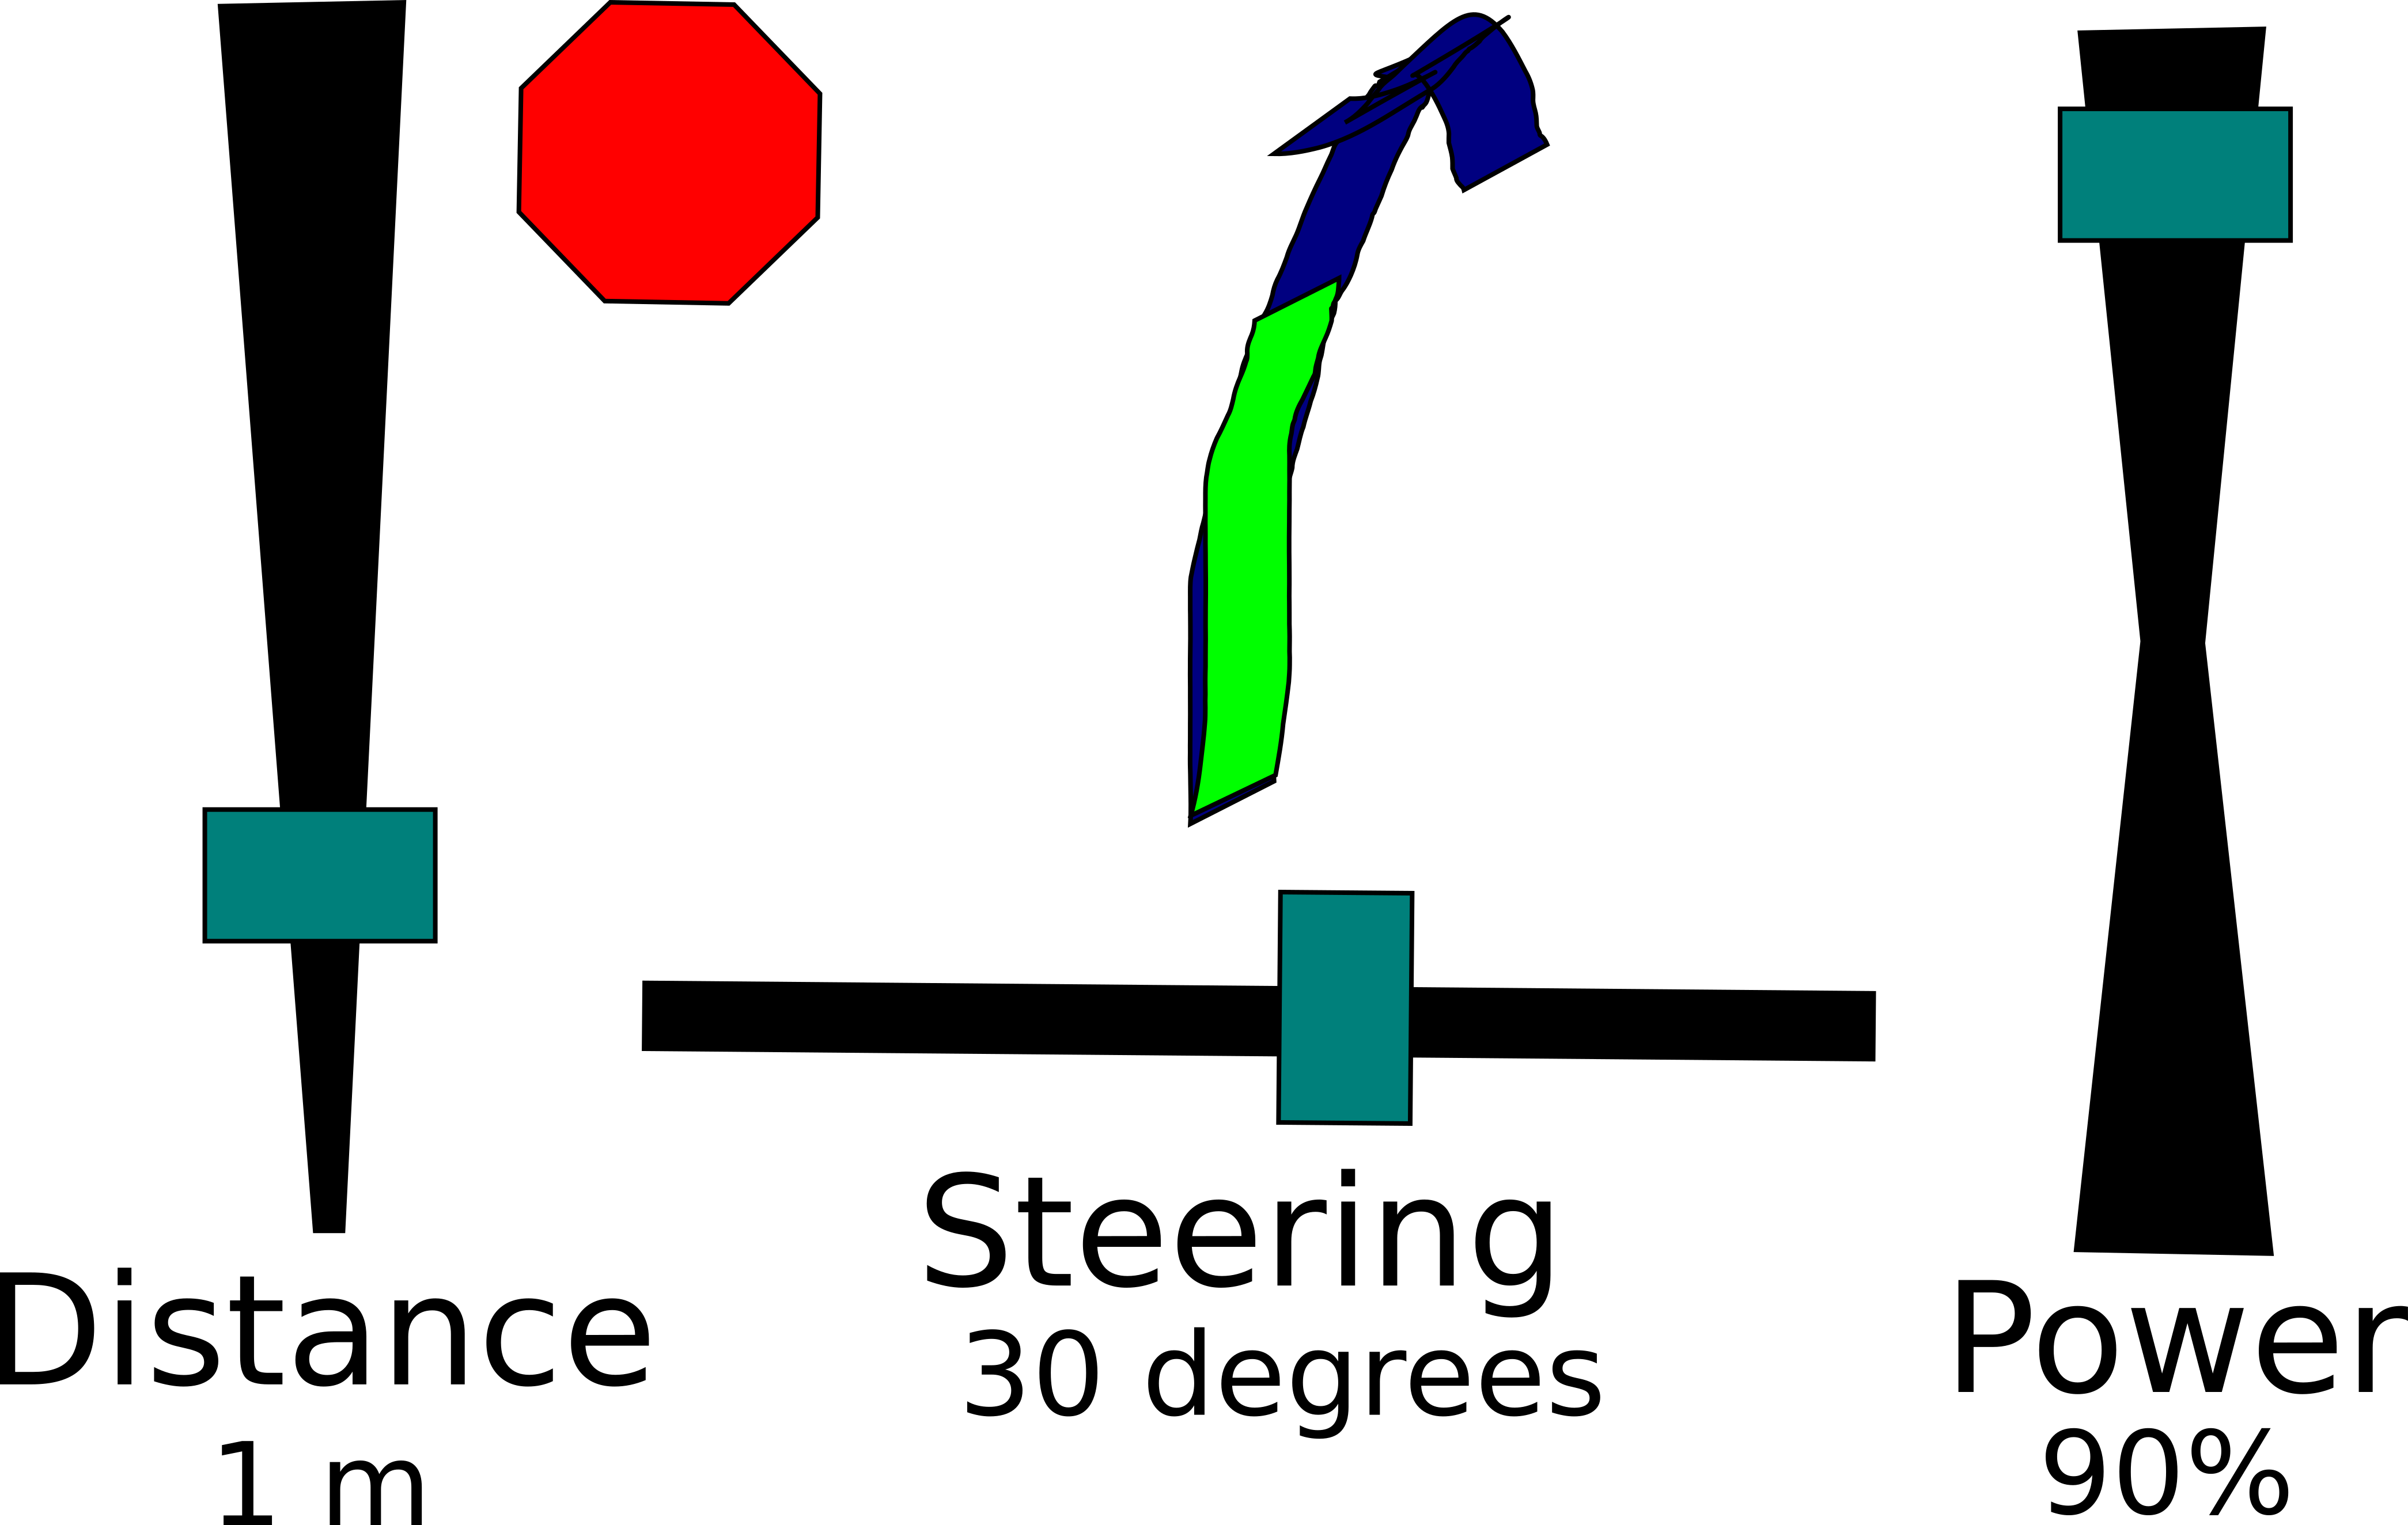
\includegraphics[width=8cm]{seperated_turning_running}
    
    Here the commanded movement is to move through 30 degrees of rotation to the right while moving 1 meter.  Note that this is what might be seen about two-thirds through the execution of the command as the stop button is visible and the path arrow is being filled in.  It would also be possible (perhaps even beneficial) to place a graphic of the rover at the current location one the arrow.
    
    This interface would also (as mentioned above) allow for commanding a pivot by simply setting the distance to zero:
    
    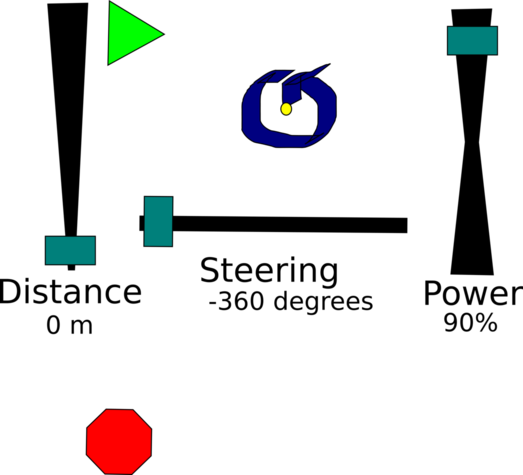
\includegraphics[width=8cm]{seperated_pivot}
    
    What might be important for displaying a pivot command, however, is to change the way that the arrow is displayed by placing a center point or something.  Or, maybe, it wouldn't matter after all.  The real question is how intuitive the arrow display is for pivoting the rover.  Of course, while this example shows a full pivot of 360 degrees to the left, it would be possible to pivot any amount.
    
    It is worth noting that even if another interface is used for the general public, this interface could still be the interface for an ``advanced'' mode.  All that would be required is to figure out what the commands to send to the rovers need to look like which would allow for both options and then to write HTML/JavaScript to implement both.  The advance interface can easily be hidden with a configuration on the rover to ensure that general public will not accidentally end up with an interface that is more difficult than desired.
    
  \subsection{Point-to-point Arc}
    This interface allows the user to select a path that is a segment of an arc between two different points.  A circle on the screen is mapped to a circle around the physical rover.  This interface would allow for controlling the rover in steering and distance in a very simple manner.  The same ``drive'' and ``stop'' buttons, as well as progress indication are applicable to this interface.  What is different is the use of a local map to select a rover path.  This interface may look something like the following:
    
    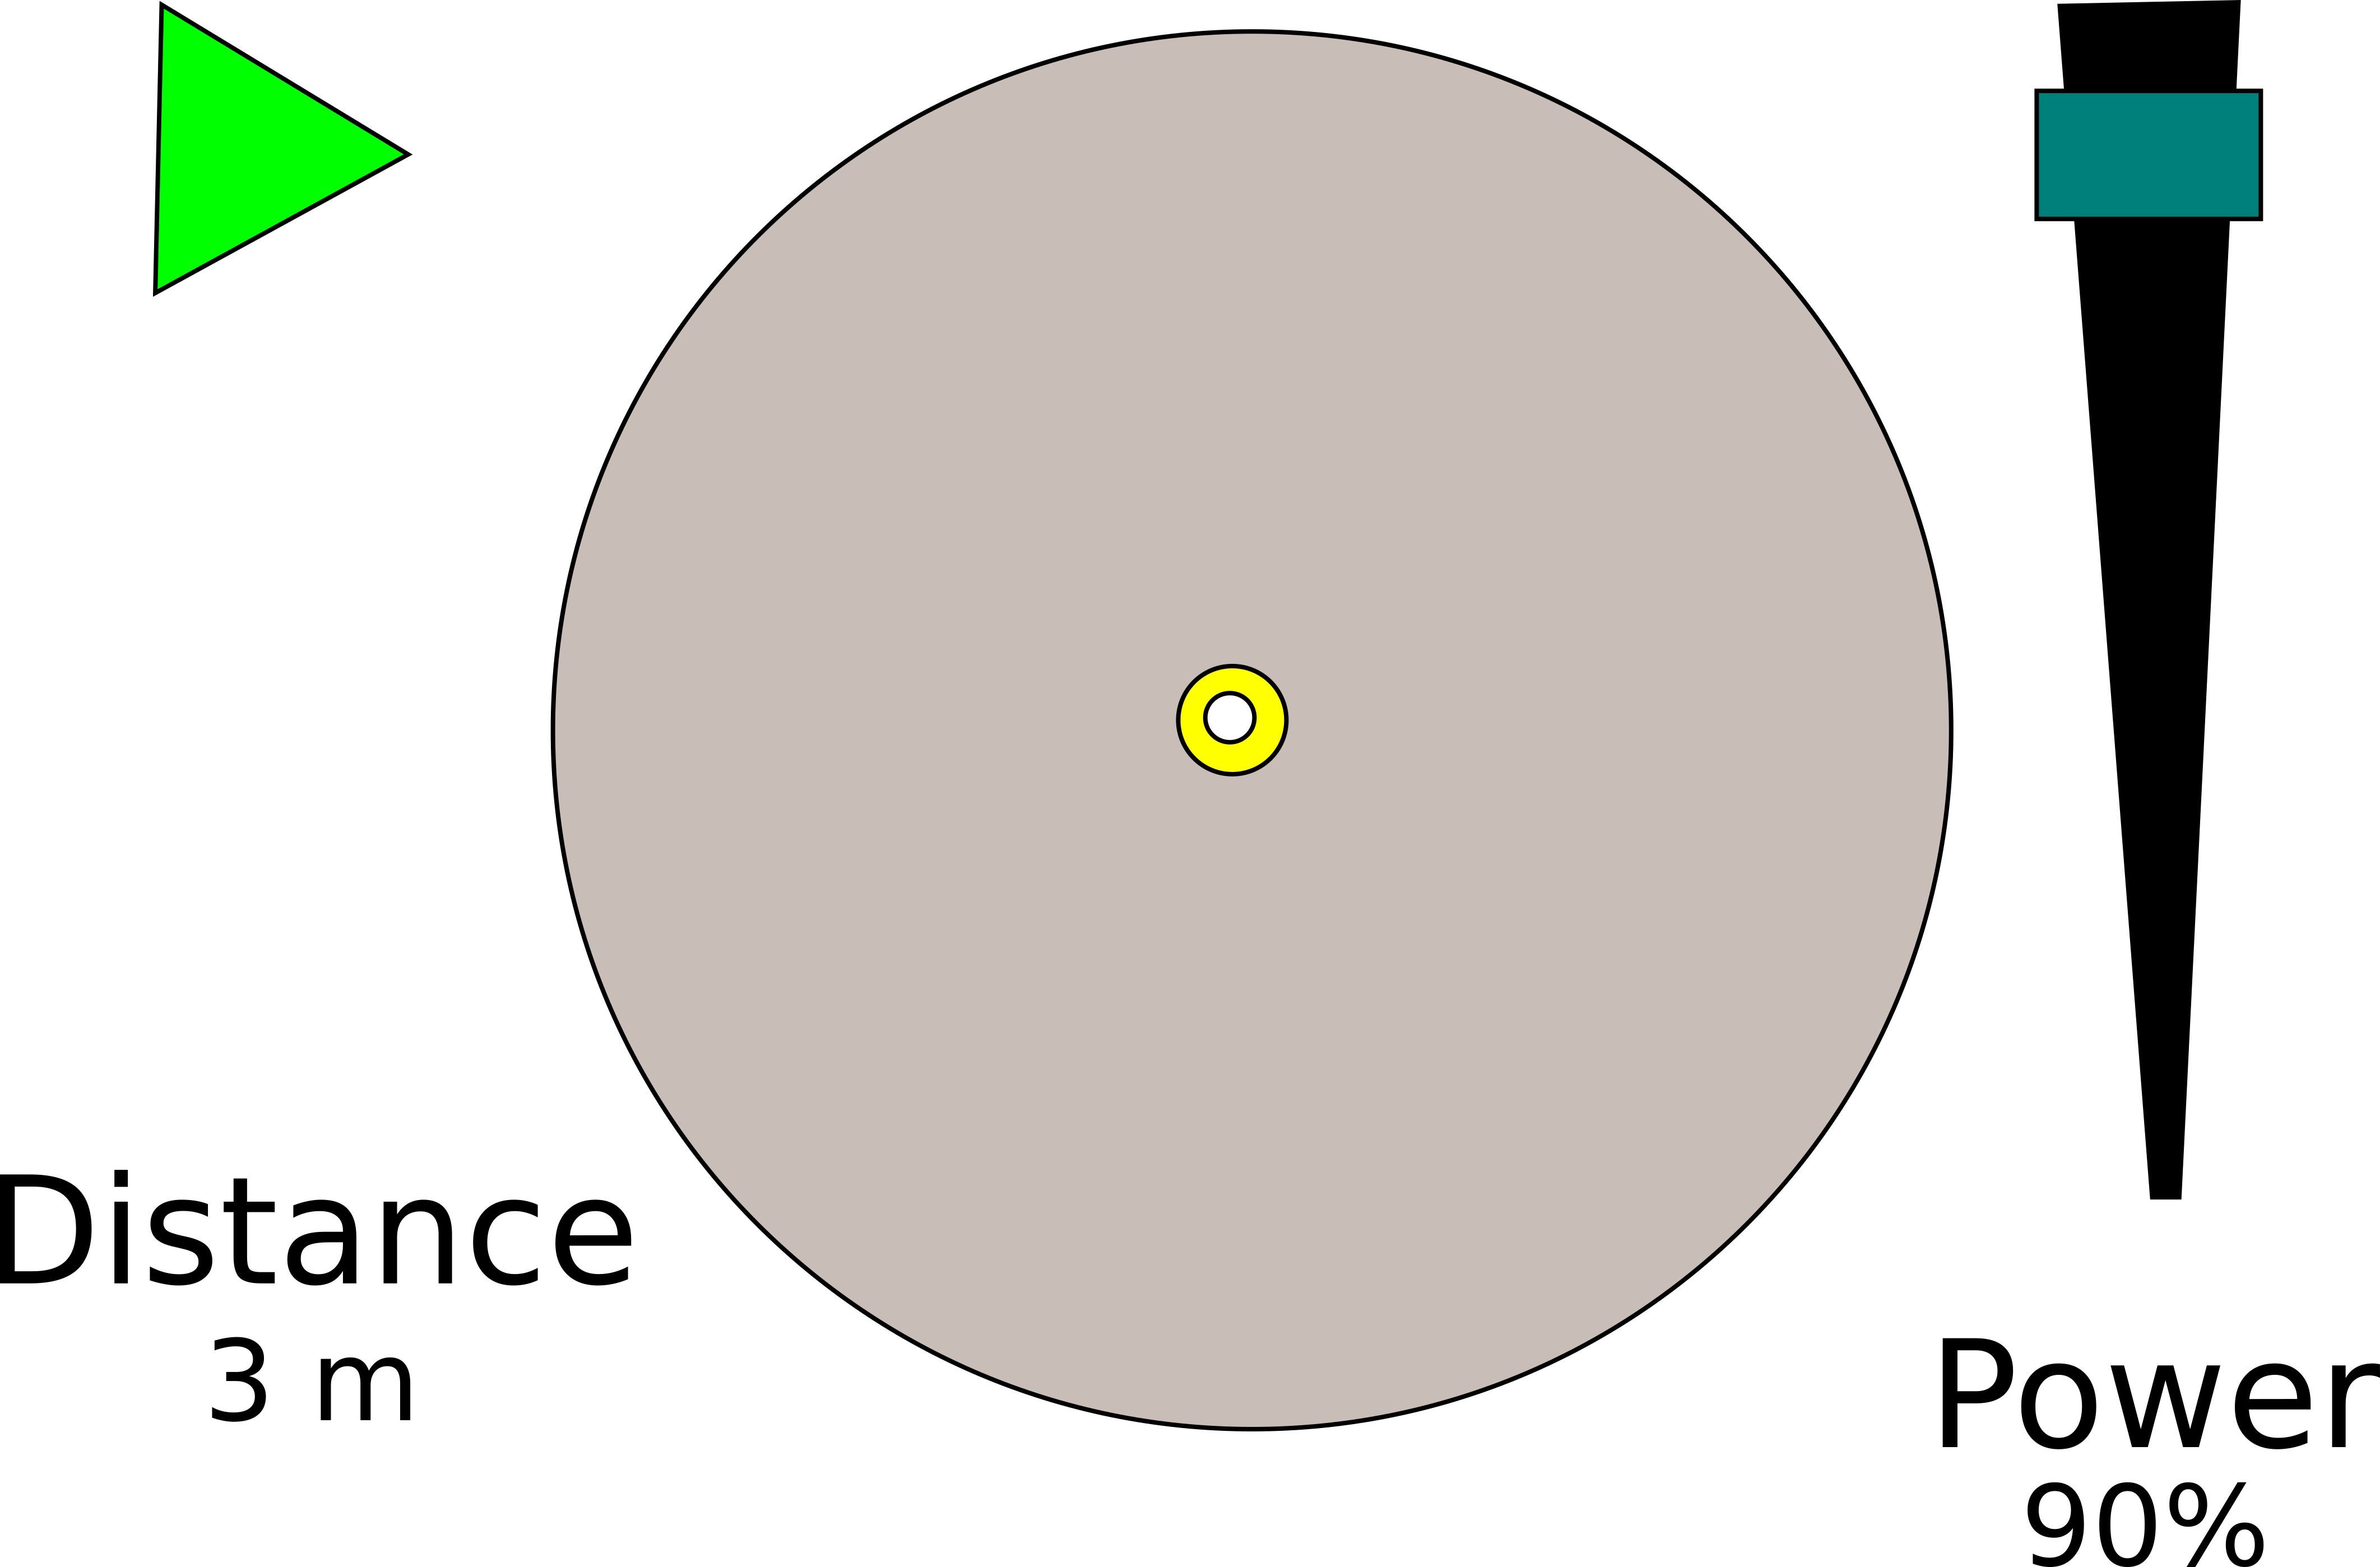
\includegraphics[width=8cm]{basic_arc}
    
    There is a large circular area which represents the immediate local neighborhood of the rover (with the rover in the center).  Clicking anywhere in the circle will set up a movement.  It is not just a straight line connection however.  As you click closer to the horizontal line, the rover will come closer to turning around complete and exactly on the horizontal, the rover will turn around 180 degrees.  The start location and direction would be connected to the end location and direction with a circular section.
    
    Straight ahead or behind, the rover will not turn:
    
    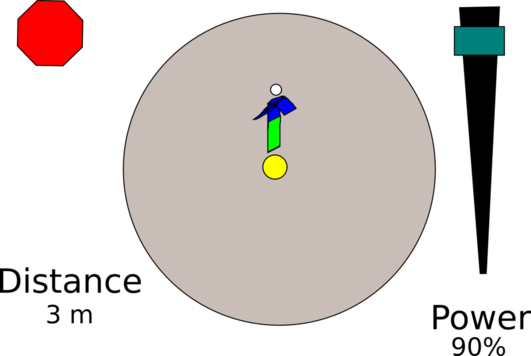
\includegraphics[width=8cm]{basic_arc_forward_running}
    
    As with the separated interface, there are built-in limits to how far the rover can be commanded to travel.  This reduces some of the major failure modes and makes success more likely.  Moreover, this ``local map'' interface would be ideal for drawing obstacles on top of if the rover had the ability to identify them.
    
    Taking a look at the circular arc fitting, we can see that it is possible to turn any amount up to 180 degrees in a single command:
    
    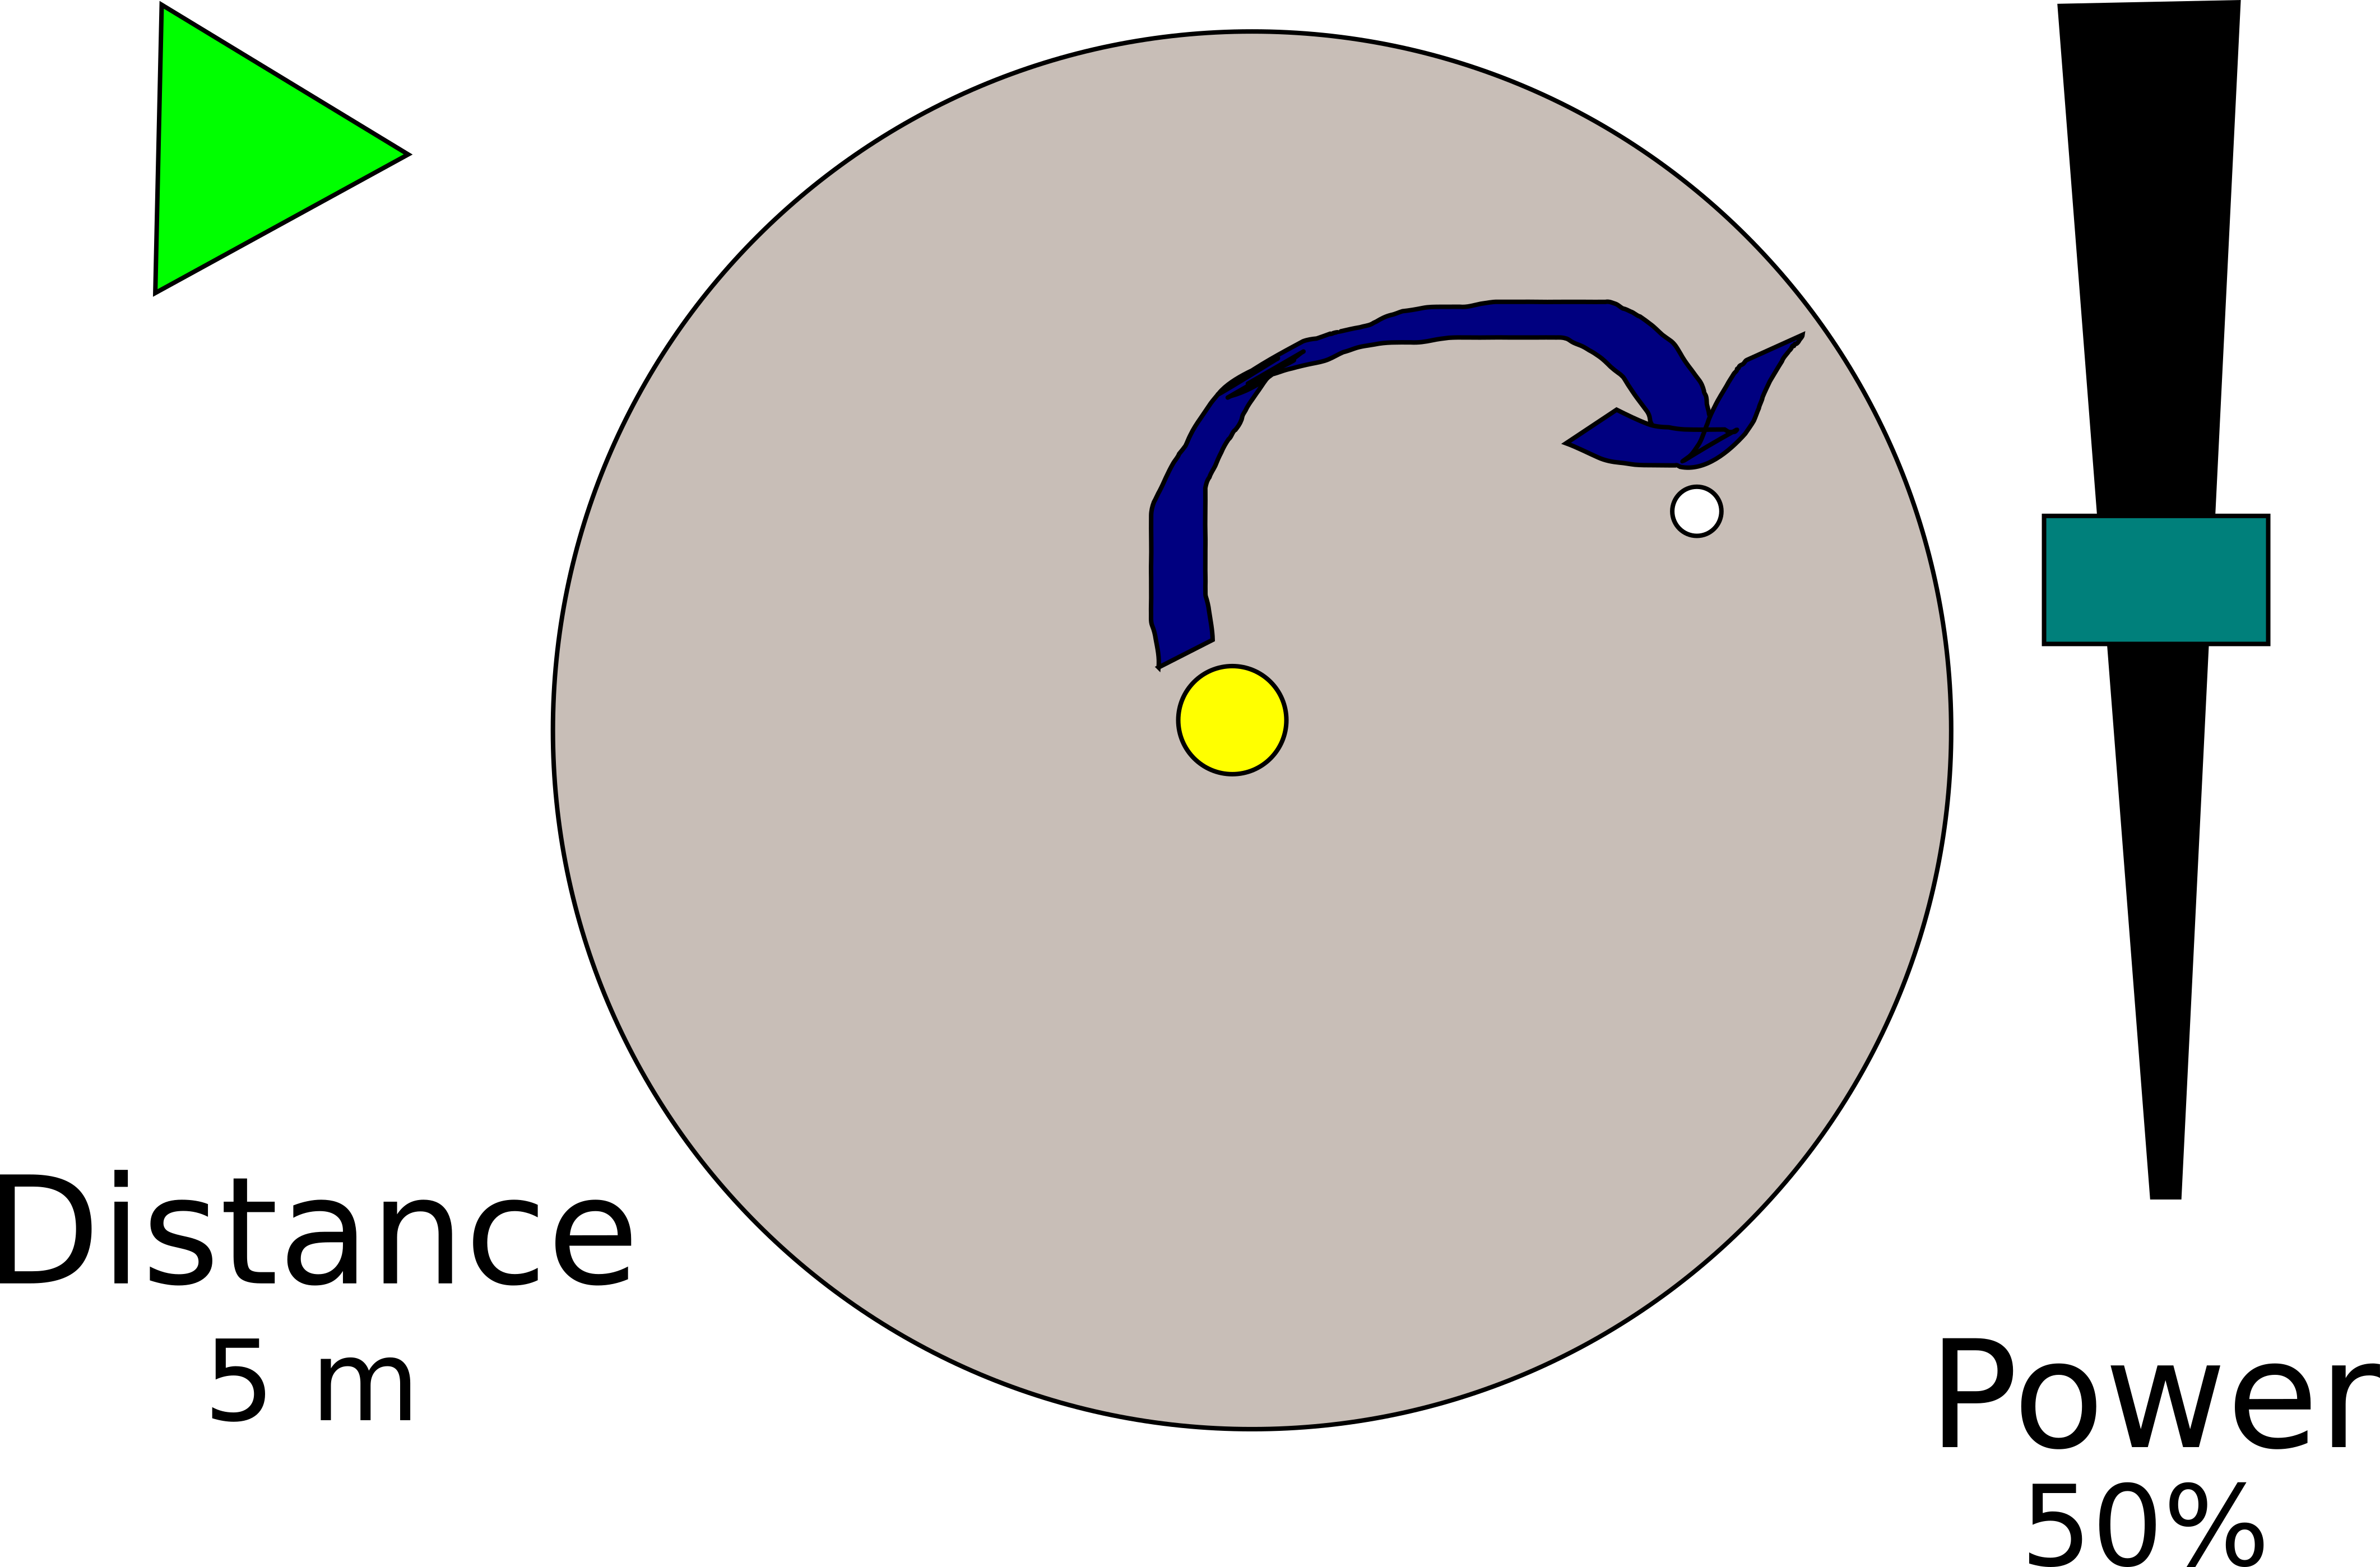
\includegraphics[width=8cm]{basic_arc_turning}
    
    At the same time, ther will always be translation in this design.
    
    
    %
\includegraphics[width=8cm]{basic_arc_reverse_turn_running}
    %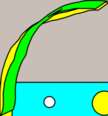
\includegraphics[width=8cm]{basic_arc_pivot_running}
    %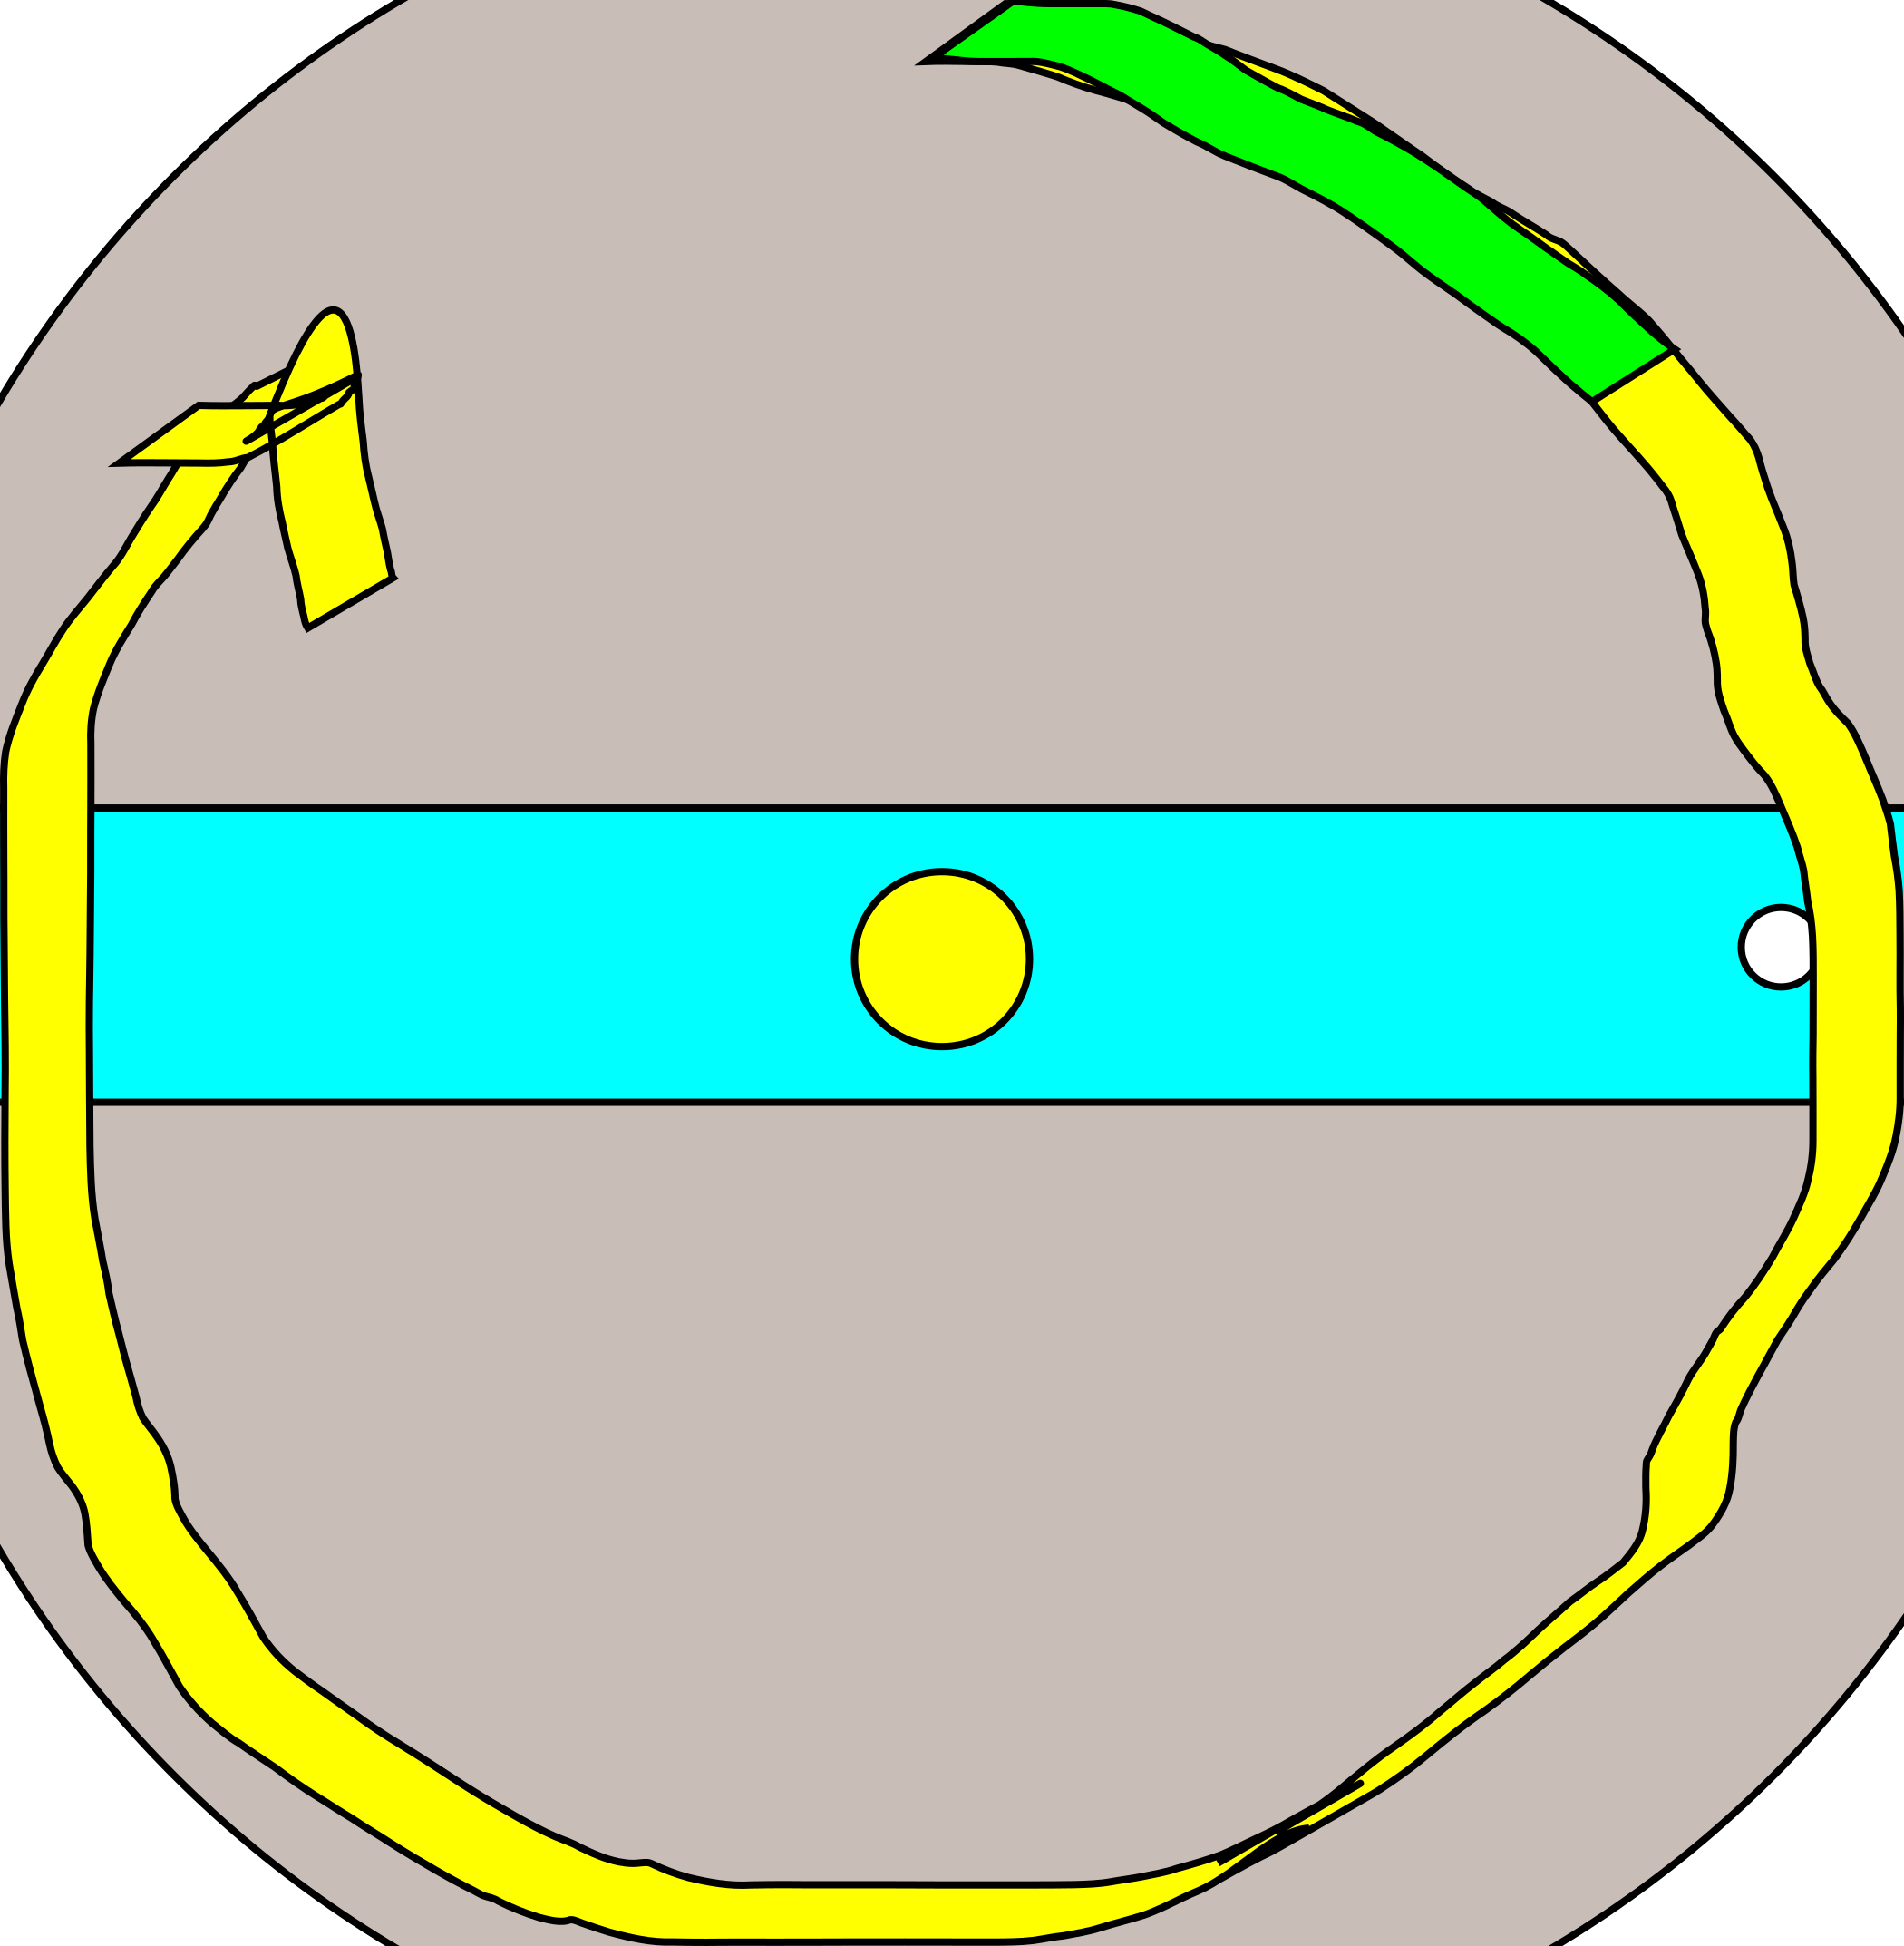
\includegraphics[width=8cm]{basic_arc_pivot_more_running}
    
    If a turn-in-place functionality is required, this would need to achieve it some other way.  Certianly, it is possible to command a tight turn with very little travel, but that is different from being able to actually command a zero-translation pivot.  Thought needs to be put into the question of if it is reasonable to provide yet another control just for pivot.  Particularly, the added control available may not warrant the added complexity of such an addition.
    
    This control would likely need to use a seperate power control of some sort if power control is desired.  It is unclear how power could be integrated smoothly onto the same interface field.  The power control could also be removed such that motor power was an autonomous function of the rover which minimized the slippage of the wheels.
    
  \subsection{Fused Point-to-point Arc with In-Place Rotation}
    This is a modified version of the last basic interface which adds a section of the control to command a turn in place.  Just like the previous interface, forward driving and turning through arcs is supported.  Along the horizontal axis, however, it is possible to command the rover to rotate in place.  This has the advantage of changing the rover's orientation without requiring any translation.  Given that much of the functionality of this interface is identical to the last one, we shall only show examples of how it is different.
    
    The horizontal band through the center of the control area specifies a pure rotation without translation.  Distance from the center denotes total angular displacement -- up to one full rotation.  For instance, a small rotation around the center could be commanded like this:
    
    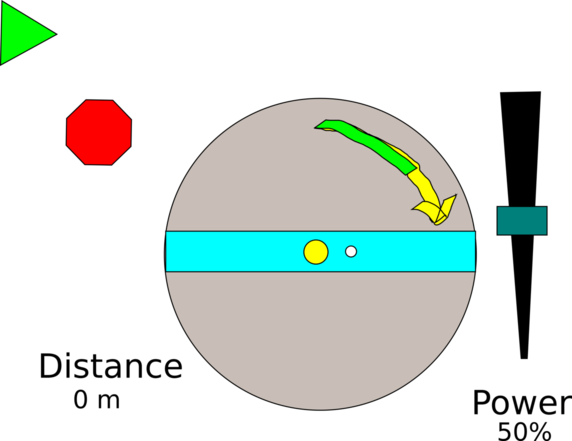
\includegraphics[width=8cm]{fused_arc_pivot}
    
    The small displacement is proportional to the distance from the center.
    
    
    This proportionality works all the way up to a full rotation as we can see in this almost complete rotation:
    
    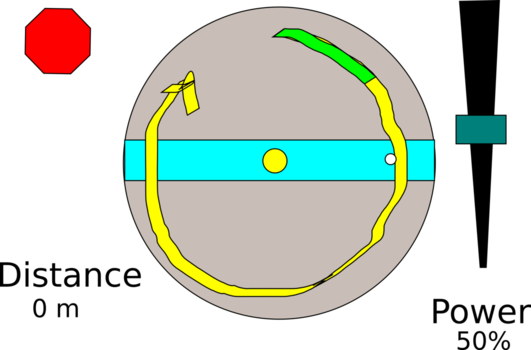
\includegraphics[width=8cm]{fused_arc_pivot_more}    
    
    It would be necessary to guarantee that the index point is on top of the rotation arrow so that it does not get lost under it.  Also, it is important to note that drawing the ``rotation'' arrows in a different color than the ``drive'' arrows makes lots of sense as it would make it less likely that people confuse different commands.
  
\section{Future Additions}
  \subsection{Command Timeouts and Override}
    If a rover is unable to complete a commanded movement within a specified time it would be helpful to make the rover simply timeout and stop trying.  It would also be good to make it possible to override an already commanded movement.  The first of these -- timeout -- would reduce rovers being placed in positions that are damaging.  The second would solve the problem of the rovers becoming non-responsive.
    
  \subsection{Advanced Mode}
    The ultimate goal of determining a new control methodology is to find a method of driving the rovers that will be easier for the general public, especially for younger children.  At the same time, it is valuable to not lose the educational potential of the current rovers.  It may be valuable to provide an ``advanced'' mode that is very similar to the current control system and is based on explicit numeric values.  It would be possible to go further too, and to provide some programmablility that is not currently available.  For instance, it would be possible to control the rover using a Python console or something similar.  If this were provided, it would be easy to use the rovers with all levels of students.
    
  \subsection{Inertial Measurement Unit (IMU)}
    While this is included in the section of potential measurements, it seems like this is so useful as to be silly to not include.  The IMU would not be visible or avaliable to the user except, perhaps, in the advanced mode (as described above).  Essentially, the IMU would be used to do more accurate closed-loop control of the rover and ensure that it follows the commanded trajectory as accurately as possible.  For all intents and purposes, the author believes that this should be treated as a necessary feature in addition to the wheel odometery sensors.
    
  \subsection{Camera}
    Since the very beginning of mobile rovers on Mars, cameras have been standard equipment.  The fact that the current rovers do not include a camera seems a major oversight.  If the control systems is based on a Raspberry Pi, this oversight can be delt with inexpensively by simply using a Raspberry Pi camera.  This addition would add to both the perceived ``coolness'' of the rovers and would make navigation easier in many cases too.
  
  \subsection{Sensor Skirt}
    The current rovers have no ability to sense their environments and return that data to the users.  This leads to some situations where it is easy to get the rover stuck and it is also far from an accurate simulation of Mars rover interactions.  A very simple addition would be a ``skirt'' of range sensors around (at least) the front of the rover to return information about how far away obstacles are.  Another option for implementing this would be to use optical techniques on the cameras to do depth estimation.  While such optical depth estimation would potentially be less expensive and more productive, it is also much more complicated and would be more difficult to implement.
    
    There are a number of models that could be used: several sonar range sensors, a single sonar range sensor, a LIDAR sensor, or optical methods.  Any of these could provide data that is superimposed on the control interface to show where the rover is capable of moving without collision.  By doing this, it would be easier for users to drive the rovers successfully.
    
  \subsection{Autonomous Control}
    Ideally, and especially if the robot posesses a sensor skirt, it would be possible to add the ability for the rovers to act at least partially autonomously.  As a bare minimum, providing the ability to avoid obtacles would be beneficial.  There is little reason not to provide such functionality if the sensor skirt is available.  There is no particular reason that the user should have any control of how such autonomous modes act though there should be feedback to the user explaining why a command is not being obeyed if it conflicts with autonomous avoidance behaviors.
    
    An additional autonomous function would be to reduce the rover's maximum speed in tight environments.  This would improve the users' ability to navigate when there are many obstacles around.
    
  \subsection{Programmable Latency}
    To improve the simultion of a mars rover, it would be possible to add latency to the control system.  Even if the latency was limited to ten seconds or so, it would make it clear why direct control is not the best solution for control on Mars.  This would likely only be enabled when in advanced mode.
\end{document}
